% Options for packages loaded elsewhere
\PassOptionsToPackage{unicode}{hyperref}
\PassOptionsToPackage{hyphens}{url}
\PassOptionsToPackage{dvipsnames,svgnames,x11names}{xcolor}
%
\documentclass[
  letterpaper,
  DIV=11,
  numbers=noendperiod]{scrartcl}

\usepackage{amsmath,amssymb}
\usepackage{iftex}
\ifPDFTeX
  \usepackage[T1]{fontenc}
  \usepackage[utf8]{inputenc}
  \usepackage{textcomp} % provide euro and other symbols
\else % if luatex or xetex
  \usepackage{unicode-math}
  \defaultfontfeatures{Scale=MatchLowercase}
  \defaultfontfeatures[\rmfamily]{Ligatures=TeX,Scale=1}
\fi
\usepackage{lmodern}
\ifPDFTeX\else  
    % xetex/luatex font selection
\fi
% Use upquote if available, for straight quotes in verbatim environments
\IfFileExists{upquote.sty}{\usepackage{upquote}}{}
\IfFileExists{microtype.sty}{% use microtype if available
  \usepackage[]{microtype}
  \UseMicrotypeSet[protrusion]{basicmath} % disable protrusion for tt fonts
}{}
\makeatletter
\@ifundefined{KOMAClassName}{% if non-KOMA class
  \IfFileExists{parskip.sty}{%
    \usepackage{parskip}
  }{% else
    \setlength{\parindent}{0pt}
    \setlength{\parskip}{6pt plus 2pt minus 1pt}}
}{% if KOMA class
  \KOMAoptions{parskip=half}}
\makeatother
\usepackage{xcolor}
\setlength{\emergencystretch}{3em} % prevent overfull lines
\setcounter{secnumdepth}{-\maxdimen} % remove section numbering
% Make \paragraph and \subparagraph free-standing
\makeatletter
\ifx\paragraph\undefined\else
  \let\oldparagraph\paragraph
  \renewcommand{\paragraph}{
    \@ifstar
      \xxxParagraphStar
      \xxxParagraphNoStar
  }
  \newcommand{\xxxParagraphStar}[1]{\oldparagraph*{#1}\mbox{}}
  \newcommand{\xxxParagraphNoStar}[1]{\oldparagraph{#1}\mbox{}}
\fi
\ifx\subparagraph\undefined\else
  \let\oldsubparagraph\subparagraph
  \renewcommand{\subparagraph}{
    \@ifstar
      \xxxSubParagraphStar
      \xxxSubParagraphNoStar
  }
  \newcommand{\xxxSubParagraphStar}[1]{\oldsubparagraph*{#1}\mbox{}}
  \newcommand{\xxxSubParagraphNoStar}[1]{\oldsubparagraph{#1}\mbox{}}
\fi
\makeatother

\usepackage{color}
\usepackage{fancyvrb}
\newcommand{\VerbBar}{|}
\newcommand{\VERB}{\Verb[commandchars=\\\{\}]}
\DefineVerbatimEnvironment{Highlighting}{Verbatim}{commandchars=\\\{\}}
% Add ',fontsize=\small' for more characters per line
\usepackage{framed}
\definecolor{shadecolor}{RGB}{241,243,245}
\newenvironment{Shaded}{\begin{snugshade}}{\end{snugshade}}
\newcommand{\AlertTok}[1]{\textcolor[rgb]{0.68,0.00,0.00}{#1}}
\newcommand{\AnnotationTok}[1]{\textcolor[rgb]{0.37,0.37,0.37}{#1}}
\newcommand{\AttributeTok}[1]{\textcolor[rgb]{0.40,0.45,0.13}{#1}}
\newcommand{\BaseNTok}[1]{\textcolor[rgb]{0.68,0.00,0.00}{#1}}
\newcommand{\BuiltInTok}[1]{\textcolor[rgb]{0.00,0.23,0.31}{#1}}
\newcommand{\CharTok}[1]{\textcolor[rgb]{0.13,0.47,0.30}{#1}}
\newcommand{\CommentTok}[1]{\textcolor[rgb]{0.37,0.37,0.37}{#1}}
\newcommand{\CommentVarTok}[1]{\textcolor[rgb]{0.37,0.37,0.37}{\textit{#1}}}
\newcommand{\ConstantTok}[1]{\textcolor[rgb]{0.56,0.35,0.01}{#1}}
\newcommand{\ControlFlowTok}[1]{\textcolor[rgb]{0.00,0.23,0.31}{\textbf{#1}}}
\newcommand{\DataTypeTok}[1]{\textcolor[rgb]{0.68,0.00,0.00}{#1}}
\newcommand{\DecValTok}[1]{\textcolor[rgb]{0.68,0.00,0.00}{#1}}
\newcommand{\DocumentationTok}[1]{\textcolor[rgb]{0.37,0.37,0.37}{\textit{#1}}}
\newcommand{\ErrorTok}[1]{\textcolor[rgb]{0.68,0.00,0.00}{#1}}
\newcommand{\ExtensionTok}[1]{\textcolor[rgb]{0.00,0.23,0.31}{#1}}
\newcommand{\FloatTok}[1]{\textcolor[rgb]{0.68,0.00,0.00}{#1}}
\newcommand{\FunctionTok}[1]{\textcolor[rgb]{0.28,0.35,0.67}{#1}}
\newcommand{\ImportTok}[1]{\textcolor[rgb]{0.00,0.46,0.62}{#1}}
\newcommand{\InformationTok}[1]{\textcolor[rgb]{0.37,0.37,0.37}{#1}}
\newcommand{\KeywordTok}[1]{\textcolor[rgb]{0.00,0.23,0.31}{\textbf{#1}}}
\newcommand{\NormalTok}[1]{\textcolor[rgb]{0.00,0.23,0.31}{#1}}
\newcommand{\OperatorTok}[1]{\textcolor[rgb]{0.37,0.37,0.37}{#1}}
\newcommand{\OtherTok}[1]{\textcolor[rgb]{0.00,0.23,0.31}{#1}}
\newcommand{\PreprocessorTok}[1]{\textcolor[rgb]{0.68,0.00,0.00}{#1}}
\newcommand{\RegionMarkerTok}[1]{\textcolor[rgb]{0.00,0.23,0.31}{#1}}
\newcommand{\SpecialCharTok}[1]{\textcolor[rgb]{0.37,0.37,0.37}{#1}}
\newcommand{\SpecialStringTok}[1]{\textcolor[rgb]{0.13,0.47,0.30}{#1}}
\newcommand{\StringTok}[1]{\textcolor[rgb]{0.13,0.47,0.30}{#1}}
\newcommand{\VariableTok}[1]{\textcolor[rgb]{0.07,0.07,0.07}{#1}}
\newcommand{\VerbatimStringTok}[1]{\textcolor[rgb]{0.13,0.47,0.30}{#1}}
\newcommand{\WarningTok}[1]{\textcolor[rgb]{0.37,0.37,0.37}{\textit{#1}}}

\providecommand{\tightlist}{%
  \setlength{\itemsep}{0pt}\setlength{\parskip}{0pt}}\usepackage{longtable,booktabs,array}
\usepackage{calc} % for calculating minipage widths
% Correct order of tables after \paragraph or \subparagraph
\usepackage{etoolbox}
\makeatletter
\patchcmd\longtable{\par}{\if@noskipsec\mbox{}\fi\par}{}{}
\makeatother
% Allow footnotes in longtable head/foot
\IfFileExists{footnotehyper.sty}{\usepackage{footnotehyper}}{\usepackage{footnote}}
\makesavenoteenv{longtable}
\usepackage{graphicx}
\makeatletter
\def\maxwidth{\ifdim\Gin@nat@width>\linewidth\linewidth\else\Gin@nat@width\fi}
\def\maxheight{\ifdim\Gin@nat@height>\textheight\textheight\else\Gin@nat@height\fi}
\makeatother
% Scale images if necessary, so that they will not overflow the page
% margins by default, and it is still possible to overwrite the defaults
% using explicit options in \includegraphics[width, height, ...]{}
\setkeys{Gin}{width=\maxwidth,height=\maxheight,keepaspectratio}
% Set default figure placement to htbp
\makeatletter
\def\fps@figure{htbp}
\makeatother

\usepackage{fvextra}
\DefineVerbatimEnvironment{Highlighting}{Verbatim}{breaklines,commandchars=\\\{\}}
\KOMAoption{captions}{tableheading}
\makeatletter
\@ifpackageloaded{caption}{}{\usepackage{caption}}
\AtBeginDocument{%
\ifdefined\contentsname
  \renewcommand*\contentsname{Table of contents}
\else
  \newcommand\contentsname{Table of contents}
\fi
\ifdefined\listfigurename
  \renewcommand*\listfigurename{List of Figures}
\else
  \newcommand\listfigurename{List of Figures}
\fi
\ifdefined\listtablename
  \renewcommand*\listtablename{List of Tables}
\else
  \newcommand\listtablename{List of Tables}
\fi
\ifdefined\figurename
  \renewcommand*\figurename{Figure}
\else
  \newcommand\figurename{Figure}
\fi
\ifdefined\tablename
  \renewcommand*\tablename{Table}
\else
  \newcommand\tablename{Table}
\fi
}
\@ifpackageloaded{float}{}{\usepackage{float}}
\floatstyle{ruled}
\@ifundefined{c@chapter}{\newfloat{codelisting}{h}{lop}}{\newfloat{codelisting}{h}{lop}[chapter]}
\floatname{codelisting}{Listing}
\newcommand*\listoflistings{\listof{codelisting}{List of Listings}}
\makeatother
\makeatletter
\makeatother
\makeatletter
\@ifpackageloaded{caption}{}{\usepackage{caption}}
\@ifpackageloaded{subcaption}{}{\usepackage{subcaption}}
\makeatother

\ifLuaTeX
  \usepackage{selnolig}  % disable illegal ligatures
\fi
\usepackage{bookmark}

\IfFileExists{xurl.sty}{\usepackage{xurl}}{} % add URL line breaks if available
\urlstyle{same} % disable monospaced font for URLs
\hypersetup{
  pdftitle={Problem Set 4},
  colorlinks=true,
  linkcolor={blue},
  filecolor={Maroon},
  citecolor={Blue},
  urlcolor={Blue},
  pdfcreator={LaTeX via pandoc}}


\title{Problem Set 4}
\author{}
\date{}

\begin{document}
\maketitle

\RecustomVerbatimEnvironment{verbatim}{Verbatim}{
  showspaces = false,
  showtabs = false,
  breaksymbolleft={},
  breaklines
}


\textbf{PS4:} Due Sat Nov 2 at 5:00PM Central. Worth 100 points. We use
(\texttt{*}) to indicate a problem that we think might be time
consuming.

\subsection{Style Points (10 pts)}\label{style-points-10-pts}

Please refer to the minilesson on code style
\textbf{\href{https://uchicago.zoom.us/rec/share/pG_wQ-pHTQrJTmqNn4rcrw5V194M2H2s-2jdy8oVhWHkd_yZt9o162IWurpA-fxU.BIQlSgZLRYctvzp-}{here}}.

\subsection{Submission Steps (10 pts)}\label{submission-steps-10-pts}

\begin{enumerate}
\def\labelenumi{\arabic{enumi}.}
\tightlist
\item
  This problem set is a paired problem set.
\item
  Play paper, scissors, rock to determine who goes first. Call that
  person \emph{Partner 1}.

  \begin{itemize}
  \tightlist
  \item
    Partner 1 (name and cnet ID): Katika Klinkaew, katikak
  \item
    Partner 2 (name and cnet ID): Liujun Hua, liujunh
  \end{itemize}
\item
  Partner 1 will accept the \texttt{ps4} and then share the link it
  creates with their partner. You can only share it with one partner so
  you will not be able to change it after your partner has accepted.
\item
  ``This submission is our work alone and complies with the 30538
  integrity policy.'' Add your initials to indicate your agreement:
  ***KK** ***LH**
\item
  ``I have uploaded the names of anyone else other than my partner and I
  worked with on the problem set
  \textbf{\href{https://docs.google.com/forms/d/185usrCREQaUbvAXpWhChkjghdGgmAZXA3lPWpXLLsts/edit}{here}}''
  (1 point)
\item
  Late coins used this pset: ***0** Late coins left after submission:
  **\_\_**
\item
  Knit your \texttt{ps4.qmd} to an PDF file to make \texttt{ps4.pdf},

  \begin{itemize}
  \tightlist
  \item
    The PDF should not be more than 25 pages. Use \texttt{head()} and
    re-size figures when appropriate.
  \end{itemize}
\item
  (Partner 1): push \texttt{ps4.qmd} and \texttt{ps4.pdf} to your github
  repo.
\item
  (Partner 1): submit \texttt{ps4.pdf} via Gradescope. Add your partner
  on Gradescope.
\item
  (Partner 1): tag your submission in Gradescope
\end{enumerate}

\textbf{Important:} Repositories are for tracking code. \textbf{Do not
commit the data or shapefiles to your repo.} The best way to do this is
with \texttt{.gitignore}, which we have covered in class. If you do
accidentally commit the data, Github has a
\href{https://docs.github.com/en/repositories/working-with-files/managing-large-files/about-large-files-on-github\#removing-files-from-a-repositorys-history}{guide}.
The best course of action depends on whether you have pushed yet. This
also means that both partners will have to download the initial raw data
and any data cleaning code will need to be re-run on both partners'
computers.

\begin{Shaded}
\begin{Highlighting}[]
\ImportTok{import}\NormalTok{ pandas }\ImportTok{as}\NormalTok{ pd}
\ImportTok{import}\NormalTok{ altair }\ImportTok{as}\NormalTok{ alt}
\ImportTok{import}\NormalTok{ os}
\ImportTok{import}\NormalTok{ warnings}
\NormalTok{warnings.filterwarnings(}\StringTok{\textquotesingle{}ignore\textquotesingle{}}\NormalTok{)}
\NormalTok{alt.renderers.enable(}\StringTok{"png"}\NormalTok{)}
\end{Highlighting}
\end{Shaded}

\begin{verbatim}
RendererRegistry.enable('png')
\end{verbatim}

\subsection{Download and explore the Provider of Services (POS) file (10
pts)}\label{download-and-explore-the-provider-of-services-pos-file-10-pts}

\begin{enumerate}
\def\labelenumi{\arabic{enumi}.}
\tightlist
\item
\end{enumerate}

\begin{verbatim}
PRVDR_CTGRY_SBTYP_CD = Sub-type of Provider
PRVDR_CTGRY_CD = Provider Category Code
PRVDR_NUM = CMS Certification Number
PGM_TRMNTN_CD = Termination Code
TRMNTN_EXPRTN_DT = Date the provider was terminated 
FAC_NAME = Facility Name
ZIP_CD = Zip code
STATE_CD = State Abbreviation
\end{verbatim}

\begin{enumerate}
\def\labelenumi{\arabic{enumi}.}
\setcounter{enumi}{1}
\tightlist
\item
  \begin{enumerate}
  \def\labelenumii{\alph{enumii}.}
  \tightlist
  \item
  \end{enumerate}
\end{enumerate}

\begin{Shaded}
\begin{Highlighting}[]
\CommentTok{\# set path and read in the pos2016.csv file}
\NormalTok{pset\_path }\OperatorTok{=} \StringTok{\textquotesingle{}/Users/katikaklinkaew/Documents/GitHub/problem{-}set{-}4{-}katika{-}and{-}liujun/data/\textquotesingle{}}

\CommentTok{\# create a function to load, filter, and count number of short{-}term hospitals}
\KeywordTok{def}\NormalTok{ read\_short\_term\_hospitals(year, pset\_path):}
    \CommentTok{"""}
\CommentTok{    read the provider{-}of{-}service data for a given year, filters for short{-}term hospitals,}
\CommentTok{    and returns the filtered DataFrame.}

\CommentTok{    Parameters:}
\CommentTok{        year (int): The year of the data (e.g., 2017).}
\CommentTok{        pset\_path (str): The path to the directory containing the CSV files.}
\CommentTok{    """}
\NormalTok{    file\_path }\OperatorTok{=}\NormalTok{ os.path.join(pset\_path, }\SpecialStringTok{f\textquotesingle{}pos}\SpecialCharTok{\{}\NormalTok{year}\SpecialCharTok{\}}\SpecialStringTok{.csv\textquotesingle{}}\NormalTok{)}
\NormalTok{    df }\OperatorTok{=}\NormalTok{ pd.read\_csv(file\_path, encoding}\OperatorTok{=}\StringTok{\textquotesingle{}latin1\textquotesingle{}}\NormalTok{)}
\NormalTok{    df }\OperatorTok{=}\NormalTok{ df[(df[}\StringTok{\textquotesingle{}PRVDR\_CTGRY\_CD\textquotesingle{}}\NormalTok{] }\OperatorTok{==} \DecValTok{1}\NormalTok{) }\OperatorTok{\&}\NormalTok{ (df[}\StringTok{\textquotesingle{}PRVDR\_CTGRY\_SBTYP\_CD\textquotesingle{}}\NormalTok{] }\OperatorTok{==} \DecValTok{1}\NormalTok{)]}
    \BuiltInTok{print}\NormalTok{(}
        \SpecialStringTok{f\textquotesingle{}There are }\SpecialCharTok{\{}\NormalTok{df}\SpecialCharTok{.}\NormalTok{shape[}\DecValTok{0}\NormalTok{]}\SpecialCharTok{\}}\SpecialStringTok{ short{-}term hospitals reported in }\SpecialCharTok{\{}\NormalTok{year}\SpecialCharTok{\}}\SpecialStringTok{ data\textquotesingle{}}\NormalTok{)}
    \ControlFlowTok{return}\NormalTok{ df}

\CommentTok{\# import pos\_2016.csv}
\NormalTok{df\_pos2016 }\OperatorTok{=}\NormalTok{ read\_short\_term\_hospitals(}\DecValTok{2016}\NormalTok{, pset\_path)}
\end{Highlighting}
\end{Shaded}

\begin{verbatim}
There are 7245 short-term hospitals reported in 2016 data
\end{verbatim}

\begin{verbatim}
b.   
According to the American Hospital Association (https://www.aha.org/statistics/2018-01-09-fast-facts-us-hospitals-2018-pie-charts), there were 5,534 hospitals in the U.S. in total which is much lower than 7,245 considering that our data only consists of short-term hospitals. One reason could be due to the difference in definition of a hospital from each source.
\end{verbatim}

\begin{enumerate}
\def\labelenumi{\arabic{enumi}.}
\setcounter{enumi}{2}
\tightlist
\item
\end{enumerate}

\begin{Shaded}
\begin{Highlighting}[]
\CommentTok{\# repeat the steps for each year}
\NormalTok{df\_pos2017 }\OperatorTok{=}\NormalTok{ read\_short\_term\_hospitals(}\DecValTok{2017}\NormalTok{, pset\_path)}
\NormalTok{df\_pos2018 }\OperatorTok{=}\NormalTok{ read\_short\_term\_hospitals(}\DecValTok{2018}\NormalTok{, pset\_path)}
\NormalTok{df\_pos2019 }\OperatorTok{=}\NormalTok{ read\_short\_term\_hospitals(}\DecValTok{2019}\NormalTok{, pset\_path)}

\CommentTok{\# append all the pos data}
\NormalTok{df\_pos2016\_to\_2019 }\OperatorTok{=}\NormalTok{ pd.concat([df\_pos2016.assign(year}\OperatorTok{=}\DecValTok{2016}\NormalTok{), df\_pos2017.assign(}
\NormalTok{    year}\OperatorTok{=}\DecValTok{2017}\NormalTok{), df\_pos2018.assign(year}\OperatorTok{=}\DecValTok{2018}\NormalTok{), df\_pos2019.assign(year}\OperatorTok{=}\DecValTok{2019}\NormalTok{)], ignore\_index}\OperatorTok{=}\VariableTok{True}\NormalTok{)}
\end{Highlighting}
\end{Shaded}

\begin{verbatim}
There are 7260 short-term hospitals reported in 2017 data
There are 7277 short-term hospitals reported in 2018 data
There are 7303 short-term hospitals reported in 2019 data
\end{verbatim}

\begin{Shaded}
\begin{Highlighting}[]
\CommentTok{\# plot number of observations by year}
\NormalTok{observation\_by\_year }\OperatorTok{=}\NormalTok{ df\_pos2016\_to\_2019.groupby(}
    \StringTok{\textquotesingle{}year\textquotesingle{}}\NormalTok{).size().reset\_index(name}\OperatorTok{=}\StringTok{\textquotesingle{}observation\_count\textquotesingle{}}\NormalTok{)}

\NormalTok{observation\_by\_year\_plot }\OperatorTok{=}\NormalTok{ alt.Chart(observation\_by\_year).mark\_bar(size}\OperatorTok{=}\DecValTok{20}\NormalTok{).encode(}
\NormalTok{    alt.X(}\StringTok{\textquotesingle{}year:O\textquotesingle{}}\NormalTok{, title}\OperatorTok{=}\StringTok{\textquotesingle{}Year\textquotesingle{}}\NormalTok{),}
\NormalTok{    alt.Y(}\StringTok{\textquotesingle{}observation\_count:Q\textquotesingle{}}\NormalTok{, title}\OperatorTok{=}\StringTok{\textquotesingle{}Number of Observations\textquotesingle{}}\NormalTok{),}
\NormalTok{).properties(}
\NormalTok{    title}\OperatorTok{=}\StringTok{\textquotesingle{}Number of observations im Provide{-}of{-}Service file between 2016 to 2019\textquotesingle{}}\NormalTok{,}
\NormalTok{    width}\OperatorTok{=}\DecValTok{300}\NormalTok{,}
\NormalTok{    height}\OperatorTok{=}\DecValTok{300}
\NormalTok{)}

\NormalTok{observation\_label }\OperatorTok{=}\NormalTok{ observation\_by\_year\_plot.mark\_text(}
\NormalTok{    align}\OperatorTok{=}\StringTok{\textquotesingle{}left\textquotesingle{}}\NormalTok{,}
\NormalTok{    baseline}\OperatorTok{=}\StringTok{\textquotesingle{}bottom\textquotesingle{}}\NormalTok{,}
\NormalTok{    dx}\OperatorTok{={-}}\DecValTok{7}\NormalTok{,}
\NormalTok{    dy}\OperatorTok{={-}}\DecValTok{5}\NormalTok{,}
\NormalTok{    fontSize}\OperatorTok{=}\DecValTok{10}
\NormalTok{).encode(}
\NormalTok{    text}\OperatorTok{=}\StringTok{\textquotesingle{}observation\_count:Q\textquotesingle{}}
\NormalTok{)}

\NormalTok{observation\_by\_year\_plot }\OperatorTok{+}\NormalTok{ observation\_label}
\end{Highlighting}
\end{Shaded}

\includegraphics[width=4.75in,height=3.92708in]{pset4_template_files/figure-pdf/cell-5-output-1.png}

\begin{enumerate}
\def\labelenumi{\arabic{enumi}.}
\setcounter{enumi}{3}
\tightlist
\item
  \begin{enumerate}
  \def\labelenumii{\alph{enumii}.}
  \tightlist
  \item
    Plot number of unique hospitals by year
  \end{enumerate}
\end{enumerate}

\begin{Shaded}
\begin{Highlighting}[]
\NormalTok{unique\_hospital\_by\_year }\OperatorTok{=}\NormalTok{ df\_pos2016\_to\_2019.groupby(}
    \StringTok{\textquotesingle{}year\textquotesingle{}}\NormalTok{)[}\StringTok{\textquotesingle{}PRVDR\_NUM\textquotesingle{}}\NormalTok{].nunique().reset\_index(name}\OperatorTok{=}\StringTok{\textquotesingle{}unique\_hospital\_count\textquotesingle{}}\NormalTok{)}

\NormalTok{unique\_hospital\_by\_year\_plot }\OperatorTok{=}\NormalTok{ alt.Chart(unique\_hospital\_by\_year).mark\_bar(size}\OperatorTok{=}\DecValTok{20}\NormalTok{, color}\OperatorTok{=}\StringTok{\textquotesingle{}lightcoral\textquotesingle{}}\NormalTok{).encode(}
\NormalTok{    alt.X(}\StringTok{\textquotesingle{}year:O\textquotesingle{}}\NormalTok{, title}\OperatorTok{=}\StringTok{\textquotesingle{}Year\textquotesingle{}}\NormalTok{),}
\NormalTok{    alt.Y(}\StringTok{\textquotesingle{}unique\_hospital\_count:Q\textquotesingle{}}\NormalTok{, title}\OperatorTok{=}\StringTok{\textquotesingle{}Number of unique hospitals\textquotesingle{}}\NormalTok{)}
\NormalTok{).properties(}
\NormalTok{    title}\OperatorTok{=}\StringTok{\textquotesingle{}Total unique hospitals by year\textquotesingle{}}\NormalTok{,}
\NormalTok{    width}\OperatorTok{=}\DecValTok{300}\NormalTok{,}
\NormalTok{    height}\OperatorTok{=}\DecValTok{300}
\NormalTok{)}

\NormalTok{unique\_label }\OperatorTok{=}\NormalTok{ unique\_hospital\_by\_year\_plot.mark\_text(}
\NormalTok{    align}\OperatorTok{=}\StringTok{\textquotesingle{}left\textquotesingle{}}\NormalTok{,}
\NormalTok{    baseline}\OperatorTok{=}\StringTok{\textquotesingle{}bottom\textquotesingle{}}\NormalTok{,}
\NormalTok{    dx}\OperatorTok{={-}}\DecValTok{5}\NormalTok{,}
\NormalTok{    dy}\OperatorTok{={-}}\DecValTok{5}\NormalTok{,}
\NormalTok{    fontSize}\OperatorTok{=}\DecValTok{10}
\NormalTok{).encode(}
\NormalTok{    text}\OperatorTok{=}\StringTok{\textquotesingle{}unique\_hospital\_count:Q\textquotesingle{}}
\NormalTok{)}

\NormalTok{unique\_hospital\_by\_year\_plot }\OperatorTok{+}\NormalTok{ unique\_label}
\end{Highlighting}
\end{Shaded}

\includegraphics[width=3.72917in,height=3.92708in]{pset4_template_files/figure-pdf/cell-6-output-1.png}

\begin{verbatim}
b. 
\end{verbatim}

From the two plots, we can see that the number of unique hospitals is
exactly the same as the number of observations in each year. It tells us
that a hospital only appears in the data once in a specific year, that
is each row in each year represents a snapshot of a unique hospital.

\subsection{Identify hospital closures in POS file (15 pts)
(*)}\label{identify-hospital-closures-in-pos-file-15-pts}

\begin{enumerate}
\def\labelenumi{\arabic{enumi}.}
\tightlist
\item
\end{enumerate}

\begin{Shaded}
\begin{Highlighting}[]
\NormalTok{df }\OperatorTok{=}\NormalTok{ df\_pos2016\_to\_2019.copy()}

\CommentTok{\# initialize a dictionary to store termination years}
\NormalTok{termination\_years }\OperatorTok{=}\NormalTok{ \{\}}

\CommentTok{\# extract the active hospitals in 2016}
\NormalTok{active\_2016 }\OperatorTok{=}\NormalTok{ df[(df[}\StringTok{\textquotesingle{}year\textquotesingle{}}\NormalTok{] }\OperatorTok{==} \DecValTok{2016}\NormalTok{) }\OperatorTok{\&}\NormalTok{ (df[}\StringTok{\textquotesingle{}PGM\_TRMNTN\_CD\textquotesingle{}}\NormalTok{] }\OperatorTok{==} \DecValTok{0}\NormalTok{)]}

\NormalTok{active\_df }\OperatorTok{=}\NormalTok{ df[df[}\StringTok{\textquotesingle{}PRVDR\_NUM\textquotesingle{}}\NormalTok{].isin(active\_2016[}\StringTok{\textquotesingle{}PRVDR\_NUM\textquotesingle{}}\NormalTok{])]}

\CommentTok{\# group data by CMS code}
\ControlFlowTok{for}\NormalTok{ hospital, group }\KeywordTok{in}\NormalTok{ active\_df.groupby(}\StringTok{\textquotesingle{}PRVDR\_NUM\textquotesingle{}}\NormalTok{):}
    \CommentTok{\# sort records by year for this hospital}
\NormalTok{    group }\OperatorTok{=}\NormalTok{ group.sort\_values(}\StringTok{\textquotesingle{}year\textquotesingle{}}\NormalTok{)}

    \CommentTok{\# set a default termination year as None}
\NormalTok{    termination\_year }\OperatorTok{=} \VariableTok{None}

    \CommentTok{\# check each year from 2017 to 2019 for termination}
    \ControlFlowTok{for}\NormalTok{ year }\KeywordTok{in}\NormalTok{ [}\DecValTok{2017}\NormalTok{, }\DecValTok{2018}\NormalTok{, }\DecValTok{2019}\NormalTok{]:}
        \CommentTok{\# filter the data for the current year}
\NormalTok{        yearly\_data }\OperatorTok{=}\NormalTok{ group[group[}\StringTok{\textquotesingle{}year\textquotesingle{}}\NormalTok{] }\OperatorTok{==}\NormalTok{ year]}

        \CommentTok{\# if no record for the hospital in this year, mark as terminated}
        \ControlFlowTok{if}\NormalTok{ yearly\_data.empty:}
\NormalTok{            termination\_year }\OperatorTok{=}\NormalTok{ year}
            \ControlFlowTok{break}
        \CommentTok{\# if the hospital is present but not active, mark as terminated}
        \ControlFlowTok{elif}\NormalTok{ yearly\_data[}\StringTok{\textquotesingle{}PGM\_TRMNTN\_CD\textquotesingle{}}\NormalTok{].values[}\DecValTok{0}\NormalTok{] }\OperatorTok{!=} \DecValTok{0}\NormalTok{:}
\NormalTok{            termination\_year }\OperatorTok{=}\NormalTok{ year}
            \ControlFlowTok{break}

    \CommentTok{\# if a termination year was identified, store it in the dictionary}
    \ControlFlowTok{if}\NormalTok{ termination\_year:}
\NormalTok{        termination\_years[hospital] }\OperatorTok{=}\NormalTok{ termination\_year}

\CommentTok{\# convert the termination years to a DataFrame}
\NormalTok{terminate\_year\_df }\OperatorTok{=}\NormalTok{ pd.DataFrame(}\BuiltInTok{list}\NormalTok{(termination\_years.items()), columns}\OperatorTok{=}\NormalTok{[}
                                 \StringTok{\textquotesingle{}PRVDR\_NUM\textquotesingle{}}\NormalTok{, }\StringTok{\textquotesingle{}Termination\_Year\textquotesingle{}}\NormalTok{])}

\CommentTok{\# adding ZIP code information for each hospital from original dataset}
\NormalTok{closed\_hospitals\_zipcode }\OperatorTok{=}\NormalTok{ active\_df[active\_df[}\StringTok{\textquotesingle{}year\textquotesingle{}}\NormalTok{] }\OperatorTok{==} \DecValTok{2016}\NormalTok{][[}
    \StringTok{\textquotesingle{}PRVDR\_NUM\textquotesingle{}}\NormalTok{, }\StringTok{\textquotesingle{}FAC\_NAME\textquotesingle{}}\NormalTok{, }\StringTok{\textquotesingle{}ZIP\_CD\textquotesingle{}}\NormalTok{]].drop\_duplicates(}\StringTok{\textquotesingle{}PRVDR\_NUM\textquotesingle{}}\NormalTok{)}

\CommentTok{\# combine termination years with ZIP code information}
\NormalTok{closed\_hospitals }\OperatorTok{=}\NormalTok{ terminate\_year\_df.merge(}
\NormalTok{    closed\_hospitals\_zipcode, on}\OperatorTok{=}\StringTok{\textquotesingle{}PRVDR\_NUM\textquotesingle{}}\NormalTok{, how}\OperatorTok{=}\StringTok{\textquotesingle{}left\textquotesingle{}}\NormalTok{)}
\end{Highlighting}
\end{Shaded}

\begin{Shaded}
\begin{Highlighting}[]
\BuiltInTok{print}\NormalTok{(}
    \SpecialStringTok{f"}\SpecialCharTok{\{}\NormalTok{closed\_hospitals}\SpecialCharTok{.}\NormalTok{shape[}\DecValTok{0}\NormalTok{]}\SpecialCharTok{\}}\SpecialStringTok{ hospitals were active in 2016 that were suspected to have closed by 2019"}\NormalTok{)}
\end{Highlighting}
\end{Shaded}

\begin{verbatim}
174 hospitals were active in 2016 that were suspected to have closed by 2019
\end{verbatim}

\begin{enumerate}
\def\labelenumi{\arabic{enumi}.}
\setcounter{enumi}{1}
\tightlist
\item
\end{enumerate}

\begin{Shaded}
\begin{Highlighting}[]
\NormalTok{closed\_hospitals.sort\_values(}\StringTok{\textquotesingle{}FAC\_NAME\textquotesingle{}}\NormalTok{)[[}\StringTok{\textquotesingle{}FAC\_NAME\textquotesingle{}}\NormalTok{,}\StringTok{\textquotesingle{}Termination\_Year\textquotesingle{}}\NormalTok{]].head(}\DecValTok{10}\NormalTok{)}
\end{Highlighting}
\end{Shaded}

\begin{longtable}[]{@{}lll@{}}
\toprule\noalign{}
& FAC\_NAME & Termination\_Year \\
\midrule\noalign{}
\endhead
\bottomrule\noalign{}
\endlastfoot
4 & ABRAZO MARYVALE CAMPUS & 2017 \\
10 & ADVENTIST MEDICAL CENTER - CENTRAL VALLEY & 2017 \\
97 & AFFINITY MEDICAL CENTER & 2018 \\
80 & ALBANY MEDICAL CENTER / SOUTH CLINICAL CAMPUS & 2017 \\
140 & ALLEGIANCE SPECIALTY HOSPITAL OF KILGORE & 2017 \\
62 & ALLIANCE LAIRD HOSPITAL & 2019 \\
101 & ALLIANCEHEALTH DEACONESS & 2019 \\
26 & ANNE BATES LEACH EYE HOSPITAL & 2019 \\
21 & ARKANSAS VALLEY REGIONAL MEDICAL CENTER & 2017 \\
69 & BANNER CHURCHILL COMMUNITY HOSPITAL & 2017 \\
\end{longtable}

\begin{enumerate}
\def\labelenumi{\arabic{enumi}.}
\setcounter{enumi}{2}
\tightlist
\item
\end{enumerate}

\begin{Shaded}
\begin{Highlighting}[]
\CommentTok{\# count the active hospitals of each zip code every year}

\NormalTok{active\_counts }\OperatorTok{=}\NormalTok{ active\_df.groupby([}\StringTok{\textquotesingle{}year\textquotesingle{}}\NormalTok{, }\StringTok{\textquotesingle{}ZIP\_CD\textquotesingle{}}\NormalTok{])[}\StringTok{\textquotesingle{}PGM\_TRMNTN\_CD\textquotesingle{}}\NormalTok{].}\BuiltInTok{apply}\NormalTok{(}
    \KeywordTok{lambda}\NormalTok{ x: (x }\OperatorTok{==} \DecValTok{0}\NormalTok{).}\BuiltInTok{sum}\NormalTok{()).reset\_index(name}\OperatorTok{=}\StringTok{\textquotesingle{}active\_count\textquotesingle{}}\NormalTok{)}

\NormalTok{zip\_and\_close\_year }\OperatorTok{=}\NormalTok{ pd.DataFrame(closed\_hospitals.groupby(}
\NormalTok{    [}\StringTok{\textquotesingle{}ZIP\_CD\textquotesingle{}}\NormalTok{, }\StringTok{\textquotesingle{}Termination\_Year\textquotesingle{}}\NormalTok{]).size()).reset\_index()}

\NormalTok{zip\_with\_merger }\OperatorTok{=}\NormalTok{ []}

\ControlFlowTok{for}\NormalTok{ index, row }\KeywordTok{in}\NormalTok{ zip\_and\_close\_year.iterrows():}
    \BuiltInTok{zip} \OperatorTok{=}\NormalTok{ row[}\StringTok{\textquotesingle{}ZIP\_CD\textquotesingle{}}\NormalTok{]}
\NormalTok{    year }\OperatorTok{=}\NormalTok{ row[}\StringTok{\textquotesingle{}Termination\_Year\textquotesingle{}}\NormalTok{]}
    \ControlFlowTok{if}\NormalTok{ year }\OperatorTok{==} \DecValTok{2019}\NormalTok{:}
        \ControlFlowTok{continue}

\NormalTok{    zip\_data }\OperatorTok{=}\NormalTok{ active\_counts[active\_counts[}\StringTok{\textquotesingle{}ZIP\_CD\textquotesingle{}}\NormalTok{] }\OperatorTok{==} \BuiltInTok{zip}\NormalTok{]}
\NormalTok{    count\_this\_year }\OperatorTok{=}\NormalTok{ zip\_data[zip\_data[}\StringTok{\textquotesingle{}year\textquotesingle{}}\NormalTok{] }\OperatorTok{==}\NormalTok{ year][}\StringTok{\textquotesingle{}active\_count\textquotesingle{}}\NormalTok{]}
\NormalTok{    count\_next\_year }\OperatorTok{=}\NormalTok{ zip\_data[zip\_data[}\StringTok{\textquotesingle{}year\textquotesingle{}}\NormalTok{] }\OperatorTok{==}\NormalTok{ (year }\OperatorTok{+} \DecValTok{1}\NormalTok{)][}\StringTok{\textquotesingle{}active\_count\textquotesingle{}}\NormalTok{]}

    \ControlFlowTok{if} \KeywordTok{not}\NormalTok{ count\_this\_year.empty }\KeywordTok{and} \KeywordTok{not}\NormalTok{ count\_next\_year.empty:}
        \CommentTok{\# extract scalar values (there should be only one value per year now)}
\NormalTok{        count\_this\_year }\OperatorTok{=}\NormalTok{ count\_this\_year.iloc[}\DecValTok{0}\NormalTok{]}
\NormalTok{        count\_next\_year }\OperatorTok{=}\NormalTok{ count\_next\_year.iloc[}\DecValTok{0}\NormalTok{]}

        \ControlFlowTok{if}\NormalTok{ count\_this\_year }\OperatorTok{\textless{}=}\NormalTok{ count\_next\_year:}
\NormalTok{            zip\_with\_merger.append(}\BuiltInTok{zip}\NormalTok{)}
\end{Highlighting}
\end{Shaded}

\begin{verbatim}
a. How many hospitals fit this definition of potentially being a merger/acquisition?
\end{verbatim}

\begin{Shaded}
\begin{Highlighting}[]
\BuiltInTok{print}\NormalTok{(}\SpecialStringTok{f"}\SpecialCharTok{\{}\BuiltInTok{len}\NormalTok{(zip\_with\_merger)}\SpecialCharTok{\}}\SpecialStringTok{ hospitals fit this definition of potentially being a merger/acquisition."}\NormalTok{)}
\end{Highlighting}
\end{Shaded}

\begin{verbatim}
96 hospitals fit this definition of potentially being a merger/acquisition.
\end{verbatim}

\begin{verbatim}
b. After correcting for this, how many hospitals do you have left?
\end{verbatim}

\begin{Shaded}
\begin{Highlighting}[]
\CommentTok{\# filter merger hospitials}
\NormalTok{closed\_hospitals }\OperatorTok{=}\NormalTok{ closed\_hospitals[}\OperatorTok{\textasciitilde{}}\NormalTok{closed\_hospitals[}\StringTok{\textquotesingle{}ZIP\_CD\textquotesingle{}}\NormalTok{].isin(}
\NormalTok{    zip\_with\_merger)]}

\BuiltInTok{print}\NormalTok{(}
    \SpecialStringTok{f"}\SpecialCharTok{\{}\NormalTok{closed\_hospitals}\SpecialCharTok{.}\NormalTok{shape[}\DecValTok{0}\NormalTok{]}\SpecialCharTok{\}}\SpecialStringTok{ hospitals were active in 2016 that were suspected to have closed by 2019"}\NormalTok{)}
\end{Highlighting}
\end{Shaded}

\begin{verbatim}
78 hospitals were active in 2016 that were suspected to have closed by 2019
\end{verbatim}

\begin{verbatim}
c. 
\end{verbatim}

\begin{Shaded}
\begin{Highlighting}[]
\NormalTok{closed\_hospitals.sort\_values(}
    \StringTok{\textquotesingle{}FAC\_NAME\textquotesingle{}}\NormalTok{)[[}\StringTok{\textquotesingle{}FAC\_NAME\textquotesingle{}}\NormalTok{, }\StringTok{\textquotesingle{}Termination\_Year\textquotesingle{}}\NormalTok{]].head(}\DecValTok{10}\NormalTok{)}
\end{Highlighting}
\end{Shaded}

\begin{longtable}[]{@{}lll@{}}
\toprule\noalign{}
& FAC\_NAME & Termination\_Year \\
\midrule\noalign{}
\endhead
\bottomrule\noalign{}
\endlastfoot
62 & ALLIANCE LAIRD HOSPITAL & 2019 \\
101 & ALLIANCEHEALTH DEACONESS & 2019 \\
26 & ANNE BATES LEACH EYE HOSPITAL & 2019 \\
115 & BARIX CLINICS OF PENNSYLVANIA & 2019 \\
171 & BAYLOR EMERGENCY MEDICAL CENTER & 2019 \\
166 & BAYLOR SCOTT \& WHITE EMERGENCY MEDICAL CENTER ... & 2019 \\
98 & BELMONT COMMUNITY HOSPITAL & 2019 \\
67 & BIG SKY MEDICAL CENTER & 2019 \\
65 & BLACK RIVER COMMUNITY MEDICAL CENTER & 2019 \\
142 & CARE REGIONAL MEDICAL CENTER & 2019 \\
\end{longtable}

\subsection{Download Census zip code shapefile (10
pt)}\label{download-census-zip-code-shapefile-10-pt}

\begin{enumerate}
\def\labelenumi{\arabic{enumi}.}
\item
  \begin{enumerate}
  \def\labelenumii{\alph{enumii}.}
  \item
    File Type \textbar{} Information Type \textbar{}\\
    .dbf\textbar{} Attribute information \textbar{}\\
    .prj \textbar{} Coordinate Reference System (CRS) description
    \textbar{}\\
    .shp \textbar{} Geometric or Spatial data (i.e., points, polygon)
    \textbar{}\\
    .shx \textbar{} Positional index for looking up geometries
    \textbar{}\\
    .xml \textbar{} Metadata about the dataset including descriptions,
    purpose, agreement of use etc. \textbar{}
  \item
  \end{enumerate}
\end{enumerate}

\begin{Shaded}
\begin{Highlighting}[]
\NormalTok{zip\_path }\OperatorTok{=} \StringTok{\textquotesingle{}/Users/katikaklinkaew/Documents/data/gz\_2010\_us\_860\_00\_500k\textquotesingle{}}

\CommentTok{\# Print the size of each file in the folder}
\ControlFlowTok{for}\NormalTok{ dataset }\KeywordTok{in}\NormalTok{ os.listdir(zip\_path):}
\NormalTok{    file\_path }\OperatorTok{=}\NormalTok{ os.path.join(zip\_path, dataset)}
\NormalTok{    size }\OperatorTok{=}\NormalTok{ os.path.getsize(file\_path)}
    \ControlFlowTok{if}\NormalTok{ size }\OperatorTok{\textless{}} \DecValTok{1024}\NormalTok{:}
\NormalTok{        size\_str }\OperatorTok{=} \SpecialStringTok{f"}\SpecialCharTok{\{}\NormalTok{size}\SpecialCharTok{:.2f\}}\SpecialStringTok{ Bytes"}
    \ControlFlowTok{elif}\NormalTok{ size }\OperatorTok{\textless{}} \DecValTok{1024} \OperatorTok{**} \DecValTok{2}\NormalTok{:}
\NormalTok{        size\_str }\OperatorTok{=} \SpecialStringTok{f"}\SpecialCharTok{\{}\NormalTok{size}\OperatorTok{/}\DecValTok{1024}\SpecialCharTok{:.2f\}}\SpecialStringTok{ KB"}
    \ControlFlowTok{else}\NormalTok{:}
\NormalTok{        size\_str }\OperatorTok{=} \SpecialStringTok{f"}\SpecialCharTok{\{}\NormalTok{size}\OperatorTok{/}\NormalTok{(}\DecValTok{1024} \OperatorTok{**} \DecValTok{2}\NormalTok{)}\SpecialCharTok{:.2f\}}\SpecialStringTok{ MB"}

    \BuiltInTok{print}\NormalTok{(}\SpecialStringTok{f"}\SpecialCharTok{\{}\NormalTok{dataset}\SpecialCharTok{\}}\SpecialStringTok{: }\SpecialCharTok{\{}\NormalTok{size\_str}\SpecialCharTok{\}}\SpecialStringTok{"}\NormalTok{)}
\end{Highlighting}
\end{Shaded}

\begin{verbatim}
gz_2010_us_860_00_500k.prj: 165.00 Bytes
gz_2010_us_860_00_500k.shx: 258.85 KB
gz_2010_us_860_00_500k.shp: 798.74 MB
gz_2010_us_860_00_500k.dbf: 6.13 MB
gz_2010_us_860_00_500k.xml: 15.27 KB
\end{verbatim}

\begin{enumerate}
\def\labelenumi{\arabic{enumi}.}
\setcounter{enumi}{1}
\tightlist
\item
\end{enumerate}

\begin{Shaded}
\begin{Highlighting}[]
\ImportTok{import}\NormalTok{ geopandas }\ImportTok{as}\NormalTok{ gpd}
\NormalTok{shapefile\_path }\OperatorTok{=}\NormalTok{ os.path.join(zip\_path, }\StringTok{\textquotesingle{}gz\_2010\_us\_860\_00\_500k.shp\textquotesingle{}}\NormalTok{)}
\NormalTok{zip\_shp }\OperatorTok{=}\NormalTok{ gpd.read\_file(shapefile\_path)}
\end{Highlighting}
\end{Shaded}

\begin{Shaded}
\begin{Highlighting}[]
\CommentTok{\# Texas zip codes start with 733, and 750 {-} 799}
\NormalTok{zip\_tx }\OperatorTok{=}\NormalTok{ zip\_shp[zip\_shp[}\StringTok{\textquotesingle{}NAME\textquotesingle{}}\NormalTok{].}\BuiltInTok{str}\NormalTok{.startswith(}
\NormalTok{    (}\StringTok{\textquotesingle{}733\textquotesingle{}}\NormalTok{, }\StringTok{\textquotesingle{}75\textquotesingle{}}\NormalTok{, }\StringTok{\textquotesingle{}76\textquotesingle{}}\NormalTok{, }\StringTok{\textquotesingle{}77\textquotesingle{}}\NormalTok{, }\StringTok{\textquotesingle{}78\textquotesingle{}}\NormalTok{, }\StringTok{\textquotesingle{}79\textquotesingle{}}\NormalTok{))]}

\NormalTok{active\_2016[}\StringTok{\textquotesingle{}ZIP\_CD\textquotesingle{}}\NormalTok{] }\OperatorTok{=}\NormalTok{ active\_2016[}\StringTok{\textquotesingle{}ZIP\_CD\textquotesingle{}}\NormalTok{].astype(}
    \BuiltInTok{int}\NormalTok{).astype(}\BuiltInTok{str}\NormalTok{).}\BuiltInTok{str}\NormalTok{.zfill(}\DecValTok{5}\NormalTok{)}
\NormalTok{zip\_tx[}\StringTok{\textquotesingle{}NAME\textquotesingle{}}\NormalTok{] }\OperatorTok{=}\NormalTok{ zip\_tx[}\StringTok{\textquotesingle{}NAME\textquotesingle{}}\NormalTok{].astype(}\BuiltInTok{str}\NormalTok{).}\BuiltInTok{str}\NormalTok{.zfill(}\DecValTok{5}\NormalTok{)}

\NormalTok{tx\_hospitals }\OperatorTok{=}\NormalTok{ active\_2016[active\_2016[}\StringTok{\textquotesingle{}ZIP\_CD\textquotesingle{}}\NormalTok{].isin(zip\_tx[}\StringTok{\textquotesingle{}NAME\textquotesingle{}}\NormalTok{])]}

\NormalTok{tx\_hospitals\_zip }\OperatorTok{=}\NormalTok{ tx\_hospitals.groupby(}
    \StringTok{\textquotesingle{}ZIP\_CD\textquotesingle{}}\NormalTok{).size().reset\_index(name}\OperatorTok{=}\StringTok{\textquotesingle{}Number of Hospitals\textquotesingle{}}\NormalTok{)}

\NormalTok{zip\_tx }\OperatorTok{=}\NormalTok{ zip\_tx.rename(columns}\OperatorTok{=}\NormalTok{\{}\StringTok{\textquotesingle{}NAME\textquotesingle{}}\NormalTok{: }\StringTok{\textquotesingle{}ZIP\_CD\textquotesingle{}}\NormalTok{\})}

\CommentTok{\# Merge on ZIP\_CD to get Texas ZIP codes with hospital counts}
\NormalTok{tx\_hospitals\_merged }\OperatorTok{=}\NormalTok{ zip\_tx.merge(tx\_hospitals\_zip, on}\OperatorTok{=}\StringTok{\textquotesingle{}ZIP\_CD\textquotesingle{}}\NormalTok{, how}\OperatorTok{=}\StringTok{\textquotesingle{}left\textquotesingle{}}\NormalTok{)}

\NormalTok{tx\_hospitals\_merged[}\StringTok{\textquotesingle{}Number of Hospitals\textquotesingle{}}\NormalTok{] }\OperatorTok{=}\NormalTok{ tx\_hospitals\_merged[}\StringTok{\textquotesingle{}Number of Hospitals\textquotesingle{}}\NormalTok{].fillna(}
    \DecValTok{0}\NormalTok{)}
\end{Highlighting}
\end{Shaded}

\begin{Shaded}
\begin{Highlighting}[]
\NormalTok{tx\_hospitals\_merged[tx\_hospitals\_merged[}\StringTok{\textquotesingle{}Number of Hospitals\textquotesingle{}}\NormalTok{]}
                    \OperatorTok{==}\NormalTok{ tx\_hospitals\_merged[}\StringTok{\textquotesingle{}Number of Hospitals\textquotesingle{}}\NormalTok{].}\BuiltInTok{max}\NormalTok{()]}
\end{Highlighting}
\end{Shaded}

\begin{longtable}[]{@{}llllllll@{}}
\toprule\noalign{}
& GEO\_ID & ZCTA5 & ZIP\_CD & LSAD & CENSUSAREA & geometry & Number of
Hospitals \\
\midrule\noalign{}
\endhead
\bottomrule\noalign{}
\endlastfoot
472 & 8600000US77030 & 77030 & 77030 & ZCTA5 & 2.521 & POLYGON
((-95.41436 29.69445, -95.41486 29.693... & 5.0 \\
\end{longtable}

\begin{Shaded}
\begin{Highlighting}[]
\ImportTok{import}\NormalTok{ matplotlib.pyplot }\ImportTok{as}\NormalTok{ plt}

\NormalTok{plt.figure(figsize}\OperatorTok{=}\NormalTok{(}\DecValTok{10}\NormalTok{, }\DecValTok{10}\NormalTok{))}
\NormalTok{tx\_hospitals\_zip\_plot }\OperatorTok{=}\NormalTok{ tx\_hospitals\_merged.plot(}
\NormalTok{    column}\OperatorTok{=}\StringTok{\textquotesingle{}Number of Hospitals\textquotesingle{}}\NormalTok{,}
\NormalTok{    legend}\OperatorTok{=}\VariableTok{True}\NormalTok{,}
\NormalTok{    linewidth}\OperatorTok{=}\FloatTok{0.5}\NormalTok{).set\_axis\_off()}
\NormalTok{plt.title(}\StringTok{\textquotesingle{}Number of Hospitals by ZIP Codes in Texas in 2016\textquotesingle{}}\NormalTok{)}
\NormalTok{plt.show()}
\end{Highlighting}
\end{Shaded}

\begin{verbatim}
<Figure size 3000x3000 with 0 Axes>
\end{verbatim}

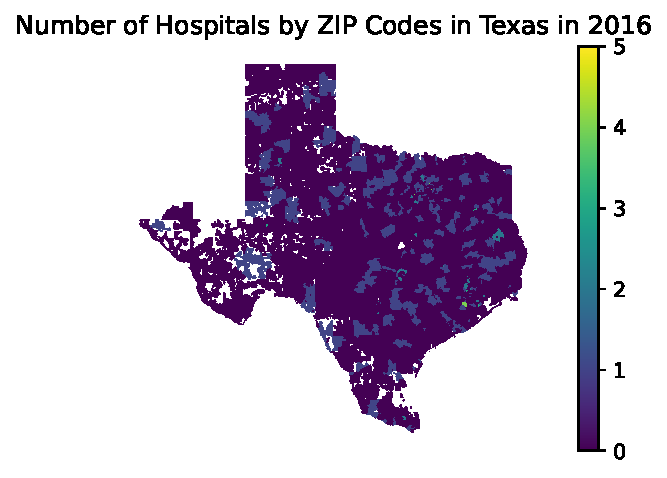
\includegraphics{pset4_template_files/figure-pdf/cell-18-output-2.pdf}

\subsection{Calculate zip code's distance to the nearest hospital (20
pts)
(*)}\label{calculate-zip-codes-distance-to-the-nearest-hospital-20-pts}

\begin{enumerate}
\def\labelenumi{\arabic{enumi}.}
\tightlist
\item
\end{enumerate}

\begin{Shaded}
\begin{Highlighting}[]
\CommentTok{\#  Create a GeoDataFrame for the centroid of each zip code nationally}
\NormalTok{zips\_all\_centroids }\OperatorTok{=}\NormalTok{ gpd.GeoDataFrame(\{}
    \StringTok{\textquotesingle{}ZIP\_CD\textquotesingle{}}\NormalTok{: zip\_shp[}\StringTok{\textquotesingle{}ZCTA5\textquotesingle{}}\NormalTok{],}
    \StringTok{\textquotesingle{}centroid\textquotesingle{}}\NormalTok{: zip\_shp.geometry.centroid}
\NormalTok{\})}

\NormalTok{zips\_all\_centroids.shape}
\end{Highlighting}
\end{Shaded}

\begin{verbatim}
(33120, 2)
\end{verbatim}

The dimensions of the GeoDataFrame include 33120 rows and 2 columns. The
first column `ZIP\_CD' is the zip codes nationally and the second column
`centroid' is the position of all the points in the zip code polygons.

\begin{enumerate}
\def\labelenumi{\arabic{enumi}.}
\setcounter{enumi}{1}
\tightlist
\item
\end{enumerate}

\begin{Shaded}
\begin{Highlighting}[]
\NormalTok{zips\_texas\_centroids }\OperatorTok{=}\NormalTok{ zips\_all\_centroids[zips\_all\_centroids[}\StringTok{\textquotesingle{}ZIP\_CD\textquotesingle{}}\NormalTok{].}\BuiltInTok{str}\NormalTok{.startswith(}
\NormalTok{    (}\StringTok{\textquotesingle{}733\textquotesingle{}}\NormalTok{, }\StringTok{\textquotesingle{}75\textquotesingle{}}\NormalTok{, }\StringTok{\textquotesingle{}76\textquotesingle{}}\NormalTok{, }\StringTok{\textquotesingle{}77\textquotesingle{}}\NormalTok{, }\StringTok{\textquotesingle{}78\textquotesingle{}}\NormalTok{, }\StringTok{\textquotesingle{}79\textquotesingle{}}\NormalTok{))]}

\CommentTok{\# the border states include NM, OK, AR, LA}
\CommentTok{\# zip codes start with 700 {-} 749, 870 {-} 884}

\NormalTok{zips\_texas\_borderstates\_centroids }\OperatorTok{=}\NormalTok{ zips\_all\_centroids[zips\_all\_centroids[}\StringTok{\textquotesingle{}ZIP\_CD\textquotesingle{}}\NormalTok{].}\BuiltInTok{str}\NormalTok{.startswith(}
\NormalTok{    (}\StringTok{\textquotesingle{}7\textquotesingle{}}\NormalTok{, }\StringTok{\textquotesingle{}87\textquotesingle{}}\NormalTok{, }\StringTok{\textquotesingle{}88\textquotesingle{}}\NormalTok{))]}

\BuiltInTok{print}\NormalTok{(}
    \SpecialStringTok{f"Unique zip codes in zip\_texas\_centroids: }\SpecialCharTok{\{}\NormalTok{zips\_texas\_centroids[}\StringTok{\textquotesingle{}ZIP\_CD\textquotesingle{}}\NormalTok{]}\SpecialCharTok{.}\NormalTok{nunique()}\SpecialCharTok{\}}\SpecialStringTok{"}\NormalTok{)}
\BuiltInTok{print}\NormalTok{(}
    \SpecialStringTok{f"Unique zip codes in zips\_texas\_borderstates\_centroids: }\SpecialCharTok{\{}\NormalTok{zips\_texas\_borderstates\_centroids[}\StringTok{\textquotesingle{}ZIP\_CD\textquotesingle{}}\NormalTok{]}\SpecialCharTok{.}\NormalTok{nunique()}\SpecialCharTok{\}}\SpecialStringTok{"}\NormalTok{)}
\end{Highlighting}
\end{Shaded}

\begin{verbatim}
Unique zip codes in zip_texas_centroids: 1935
Unique zip codes in zips_texas_borderstates_centroids: 4057
\end{verbatim}

\begin{enumerate}
\def\labelenumi{\arabic{enumi}.}
\setcounter{enumi}{2}
\tightlist
\item
  I will do a inner join merge on variables merging on ZIP\_CD.
\end{enumerate}

\begin{Shaded}
\begin{Highlighting}[]
\NormalTok{zip\_2016 }\OperatorTok{=}\NormalTok{ pd.DataFrame(active\_2016[}\StringTok{\textquotesingle{}ZIP\_CD\textquotesingle{}}\NormalTok{].fillna(}
    \DecValTok{0}\NormalTok{).astype(}\BuiltInTok{int}\NormalTok{).astype(}\BuiltInTok{str}\NormalTok{).}\BuiltInTok{str}\NormalTok{.zfill(}\DecValTok{5}\NormalTok{).drop\_duplicates())}
\NormalTok{zip\_2016.columns }\OperatorTok{=}\NormalTok{ [}\StringTok{\textquotesingle{}ZIP\_CD\textquotesingle{}}\NormalTok{]}
\NormalTok{zips\_texas\_borderstates\_centroids[}\StringTok{\textquotesingle{}ZIP\_CD\textquotesingle{}}\NormalTok{] }\OperatorTok{=}\NormalTok{ zips\_texas\_borderstates\_centroids[}\StringTok{\textquotesingle{}ZIP\_CD\textquotesingle{}}\NormalTok{].astype(}
    \BuiltInTok{str}\NormalTok{)}

\NormalTok{zips\_withhospital\_centroids }\OperatorTok{=}\NormalTok{ zips\_texas\_borderstates\_centroids.merge(}
\NormalTok{    zip\_2016, on}\OperatorTok{=}\StringTok{\textquotesingle{}ZIP\_CD\textquotesingle{}}\NormalTok{)}
\end{Highlighting}
\end{Shaded}

\begin{Shaded}
\begin{Highlighting}[]
\NormalTok{zips\_withhospital\_centroids.head(}\DecValTok{1}\NormalTok{)}
\end{Highlighting}
\end{Shaded}

\begin{longtable}[]{@{}lll@{}}
\toprule\noalign{}
& ZIP\_CD & centroid \\
\midrule\noalign{}
\endhead
\bottomrule\noalign{}
\endlastfoot
0 & 70043 & POINT (-89.96276 29.94804) \\
\end{longtable}

\begin{enumerate}
\def\labelenumi{\arabic{enumi}.}
\setcounter{enumi}{3}
\tightlist
\item
  \begin{enumerate}
  \def\labelenumii{\alph{enumii}.}
  \tightlist
  \item
    Try the join with 10 zip codes
  \end{enumerate}
\end{enumerate}

\begin{Shaded}
\begin{Highlighting}[]
\ImportTok{import}\NormalTok{ time}
\ImportTok{from}\NormalTok{ shapely.geometry }\ImportTok{import}\NormalTok{ Point}

\NormalTok{zips\_texas\_centroids }\OperatorTok{=}\NormalTok{ zips\_texas\_centroids.set\_geometry(}\StringTok{\textquotesingle{}centroid\textquotesingle{}}\NormalTok{)}
\NormalTok{zips\_withhospital\_centroids }\OperatorTok{=}\NormalTok{ zips\_withhospital\_centroids.set\_geometry(}
    \StringTok{\textquotesingle{}centroid\textquotesingle{}}\NormalTok{)}

\CommentTok{\# subset the first ten row}
\NormalTok{zips\_texas\_centroids\_subset }\OperatorTok{=}\NormalTok{ zips\_texas\_centroids[:}\DecValTok{10}\NormalTok{]}

\NormalTok{start\_time }\OperatorTok{=}\NormalTok{ time.time()}

\NormalTok{nearest\_distances }\OperatorTok{=}\NormalTok{ []}

\CommentTok{\# loop over each row in the first 10 rows of zips\_texas\_centroids}
\ControlFlowTok{for}\NormalTok{ \_, row\_tx }\KeywordTok{in}\NormalTok{ zips\_texas\_centroids\_subset.iterrows():}
\NormalTok{    point1 }\OperatorTok{=}\NormalTok{ row\_tx[}\StringTok{\textquotesingle{}centroid\textquotesingle{}}\NormalTok{]}
\NormalTok{    nearest\_distance }\OperatorTok{=} \BuiltInTok{float}\NormalTok{(}\StringTok{\textquotesingle{}inf\textquotesingle{}}\NormalTok{)  }\CommentTok{\# Initialize to a large number}

    \CommentTok{\# loop over each row in zips\_withhospital\_centroids}
    \ControlFlowTok{for}\NormalTok{ \_, row\_all }\KeywordTok{in}\NormalTok{ zips\_withhospital\_centroids.iterrows():}
\NormalTok{        point2 }\OperatorTok{=}\NormalTok{ row\_all[}\StringTok{\textquotesingle{}centroid\textquotesingle{}}\NormalTok{]}

        \CommentTok{\# calculate distance}
\NormalTok{        distance\_new }\OperatorTok{=}\NormalTok{ point1.distance(point2)}

        \CommentTok{\# update nearest distance if a closer point is found}
        \ControlFlowTok{if}\NormalTok{ distance\_new }\OperatorTok{\textless{}}\NormalTok{ nearest\_distance:}
\NormalTok{            nearest\_distance }\OperatorTok{=}\NormalTok{ distance\_new}

    \CommentTok{\# append the nearest distance for the current row in zips\_texas\_centroids}
\NormalTok{    nearest\_distances.append(nearest\_distance)}

\CommentTok{\# assign the calculated distances}
\NormalTok{zips\_texas\_centroids\_subset[}\StringTok{\textquotesingle{}nearest\_distance\textquotesingle{}}\NormalTok{] }\OperatorTok{=}\NormalTok{ nearest\_distances}

\NormalTok{end\_time }\OperatorTok{=}\NormalTok{ time.time()}

\BuiltInTok{print}\NormalTok{(}\SpecialStringTok{f"Runtime: }\SpecialCharTok{\{}\NormalTok{end\_time }\OperatorTok{{-}}\NormalTok{ start\_time}\SpecialCharTok{\}}\SpecialStringTok{"}\NormalTok{)}
\end{Highlighting}
\end{Shaded}

\begin{verbatim}
Runtime: 0.0890359878540039
\end{verbatim}

It takes around 0.13 seconds to join the 10 zip codes. As there are 1935
unique zip codes in zip\_texas\_centroids, the total would be
0.13*1935/10 = 25 seconds. In other words, we estimate the entire
procedure will take around 25 seconds.

\begin{verbatim}
b. Doing the full join
\end{verbatim}

\begin{Shaded}
\begin{Highlighting}[]
\NormalTok{start\_time }\OperatorTok{=}\NormalTok{ time.time()}

\NormalTok{nearest\_distances }\OperatorTok{=}\NormalTok{ []}

\CommentTok{\# loop over each row in zips\_texas\_centroids}
\ControlFlowTok{for}\NormalTok{ \_, row\_tx }\KeywordTok{in}\NormalTok{ zips\_texas\_centroids.iterrows():}
\NormalTok{    point1 }\OperatorTok{=}\NormalTok{ row\_tx[}\StringTok{\textquotesingle{}centroid\textquotesingle{}}\NormalTok{]}
\NormalTok{    nearest\_distance }\OperatorTok{=} \BuiltInTok{float}\NormalTok{(}\StringTok{\textquotesingle{}inf\textquotesingle{}}\NormalTok{)  }\CommentTok{\# initialize to a large number}

    \CommentTok{\# loop over each row in zips\_withhospital\_centroids}
    \ControlFlowTok{for}\NormalTok{ \_, row\_all }\KeywordTok{in}\NormalTok{ zips\_withhospital\_centroids.iterrows():}
\NormalTok{        point2 }\OperatorTok{=}\NormalTok{ row\_all[}\StringTok{\textquotesingle{}centroid\textquotesingle{}}\NormalTok{]}

        \CommentTok{\# calculate distance}
\NormalTok{        distance\_new }\OperatorTok{=}\NormalTok{ point1.distance(point2)}

        \CommentTok{\# update nearest distance if a closer point is found}
        \ControlFlowTok{if}\NormalTok{ distance\_new }\OperatorTok{\textless{}}\NormalTok{ nearest\_distance:}
\NormalTok{            nearest\_distance }\OperatorTok{=}\NormalTok{ distance\_new}

    \CommentTok{\# append the nearest distance for the current row in zips\_texas\_centroids}
\NormalTok{    nearest\_distances.append(nearest\_distance)}

\CommentTok{\# assign the calculated distances}
\NormalTok{zips\_texas\_centroids[}\StringTok{\textquotesingle{}nearest\_distance\textquotesingle{}}\NormalTok{] }\OperatorTok{=}\NormalTok{ nearest\_distances}

\NormalTok{end\_time }\OperatorTok{=}\NormalTok{ time.time()}

\BuiltInTok{print}\NormalTok{(}\SpecialStringTok{f"Runtime: }\SpecialCharTok{\{}\NormalTok{end\_time }\OperatorTok{{-}}\NormalTok{ start\_time}\SpecialCharTok{\}}\SpecialStringTok{"}\NormalTok{)}
\end{Highlighting}
\end{Shaded}

\begin{verbatim}
Runtime: 15.550760984420776
\end{verbatim}

\begin{verbatim}
c.
The unit is 'Degree'. One degree of latitude is approximately 69 miles, while one degree of longitude is approximately 54.6 miles. In this case, we will neglect longitude and multiply the degree by 69 to convert it to miles.
\end{verbatim}

\begin{Shaded}
\begin{Highlighting}[]
\CommentTok{\# convert the degree unit to miles}
\NormalTok{zips\_texas\_centroids[}\StringTok{\textquotesingle{}nearest\_distance\textquotesingle{}}\NormalTok{] }\OperatorTok{=}\NormalTok{ zips\_texas\_centroids[}\StringTok{\textquotesingle{}nearest\_distance\textquotesingle{}}\NormalTok{] }\OperatorTok{*} \DecValTok{69}
\end{Highlighting}
\end{Shaded}

\begin{enumerate}
\def\labelenumi{\arabic{enumi}.}
\setcounter{enumi}{4}
\item
  Calculate the average distance to the nearest hospital for each zip
  code in Texas

  \begin{enumerate}
  \def\labelenumii{\alph{enumii}.}
  \item
    The unit is `Miles'.
  \item
    Report the average distance in miles
  \end{enumerate}
\end{enumerate}

\begin{Shaded}
\begin{Highlighting}[]
\NormalTok{zips\_texas\_centroids[}\StringTok{\textquotesingle{}nearest\_distance\textquotesingle{}}\NormalTok{].mean()}
\end{Highlighting}
\end{Shaded}

\begin{verbatim}
np.float64(14.560206510814892)
\end{verbatim}

The average distance to the nearest hospital for each zip code in Texas
is 14.56 miles, which makes sense.

\begin{verbatim}
c. Map the value for each zip code
\end{verbatim}

\begin{Shaded}
\begin{Highlighting}[]
\NormalTok{fig, ax }\OperatorTok{=}\NormalTok{ plt.subplots()}

\CommentTok{\# Plotting the polygons from zip\_tx}
\NormalTok{zip\_tx.plot(ax}\OperatorTok{=}\NormalTok{ax, color}\OperatorTok{=}\VariableTok{None}\NormalTok{, edgecolor}\OperatorTok{=}\StringTok{"grey"}\NormalTok{, alpha}\OperatorTok{=}\FloatTok{0.5}\NormalTok{, label}\OperatorTok{=}\StringTok{"Dense"}\NormalTok{)}

\CommentTok{\# Plotting the centroids with a color gradient based on \textquotesingle{}nearest\_distance\textquotesingle{}}
\CommentTok{\# \textasciigrave{}cmap\textasciigrave{} sets the color map (e.g., \textquotesingle{}viridis\textquotesingle{}, \textquotesingle{}coolwarm\textquotesingle{}, \textquotesingle{}plasma\textquotesingle{}, etc.)}
\NormalTok{zips\_texas\_centroids.plot(}
\NormalTok{    ax}\OperatorTok{=}\NormalTok{ax,}
\NormalTok{    column}\OperatorTok{=}\StringTok{\textquotesingle{}nearest\_distance\textquotesingle{}}\NormalTok{,}
\NormalTok{    cmap}\OperatorTok{=}\StringTok{\textquotesingle{}YlGnBu\textquotesingle{}}\NormalTok{,  }\CommentTok{\# Choose a color map that suits your visualization}
\NormalTok{    alpha}\OperatorTok{=}\FloatTok{0.8}\NormalTok{,}
\NormalTok{    markersize}\OperatorTok{=}\DecValTok{20}\NormalTok{,}
\NormalTok{    legend}\OperatorTok{=}\VariableTok{True}\NormalTok{,  }\CommentTok{\# Show legend for color scale}
\NormalTok{    label}\OperatorTok{=}\StringTok{"Centroids"}
\NormalTok{)}

\CommentTok{\# Remove axis for a cleaner look}
\NormalTok{ax.set\_axis\_off()}

\CommentTok{\# Show plot}
\NormalTok{plt.show()}
\end{Highlighting}
\end{Shaded}

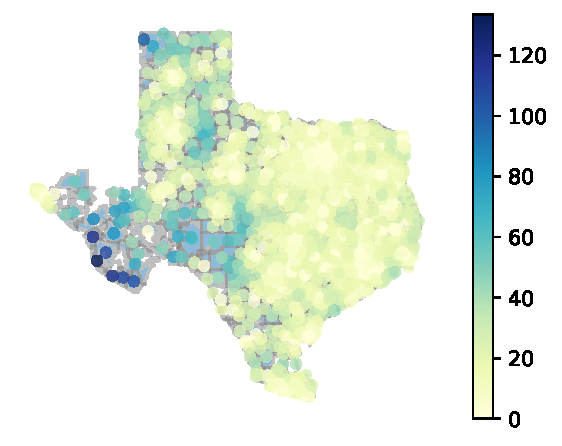
\includegraphics{pset4_template_files/figure-pdf/cell-27-output-1.pdf}

Most areas on the east side of Texas have nearby hospitals, while some
areas on the west side near the border have a much greater distance to
the nearest hospital.

\subsection{Effects of closures on access in Texas (15
pts)}\label{effects-of-closures-on-access-in-texas-15-pts}

\begin{enumerate}
\def\labelenumi{\arabic{enumi}.}
\tightlist
\item
\end{enumerate}

\begin{Shaded}
\begin{Highlighting}[]
\NormalTok{closed\_hospitals[}\StringTok{\textquotesingle{}ZIP\_CD\textquotesingle{}}\NormalTok{] }\OperatorTok{=}\NormalTok{ closed\_hospitals[}\StringTok{\textquotesingle{}ZIP\_CD\textquotesingle{}}\NormalTok{].astype(}
    \BuiltInTok{int}\NormalTok{).astype(}\BuiltInTok{str}\NormalTok{).}\BuiltInTok{str}\NormalTok{.zfill(}\DecValTok{5}\NormalTok{)}

\CommentTok{\# filter to hospital closures in Texas}
\NormalTok{closed\_hospitals\_tx }\OperatorTok{=}\NormalTok{ closed\_hospitals[closed\_hospitals[}\StringTok{\textquotesingle{}ZIP\_CD\textquotesingle{}}\NormalTok{].isin(}
\NormalTok{    zip\_tx[}\StringTok{\textquotesingle{}ZIP\_CD\textquotesingle{}}\NormalTok{])]}

\CommentTok{\# count number of hospital closures by each zip code}
\NormalTok{closed\_hospitals\_tx\_zip }\OperatorTok{=}\NormalTok{ closed\_hospitals\_tx.groupby(}
    \StringTok{\textquotesingle{}ZIP\_CD\textquotesingle{}}\NormalTok{).size().reset\_index(name}\OperatorTok{=}\StringTok{\textquotesingle{}Number of Hospital Closures\textquotesingle{}}\NormalTok{)}

\NormalTok{closed\_hospitals\_tx\_zip}
\end{Highlighting}
\end{Shaded}

\begin{longtable}[]{@{}lll@{}}
\toprule\noalign{}
& ZIP\_CD & Number of Hospital Closures \\
\midrule\noalign{}
\endhead
\bottomrule\noalign{}
\endlastfoot
0 & 75051 & 1 \\
1 & 75087 & 1 \\
2 & 75140 & 1 \\
3 & 75235 & 1 \\
4 & 75390 & 1 \\
5 & 76520 & 1 \\
6 & 76531 & 1 \\
7 & 76645 & 1 \\
8 & 77065 & 1 \\
9 & 78336 & 1 \\
10 & 78613 & 1 \\
11 & 79520 & 1 \\
12 & 79529 & 1 \\
13 & 79902 & 1 \\
\end{longtable}

\begin{enumerate}
\def\labelenumi{\arabic{enumi}.}
\setcounter{enumi}{1}
\tightlist
\item
\end{enumerate}

\begin{Shaded}
\begin{Highlighting}[]
\CommentTok{\# merge hospital closures in Texas to Texas shapefile}
\NormalTok{closed\_hospitals\_tx\_zip\_merged }\OperatorTok{=}\NormalTok{ zip\_tx.merge(}
\NormalTok{    closed\_hospitals\_tx\_zip, on}\OperatorTok{=}\StringTok{\textquotesingle{}ZIP\_CD\textquotesingle{}}\NormalTok{, how}\OperatorTok{=}\StringTok{\textquotesingle{}left\textquotesingle{}}\NormalTok{)}

\CommentTok{\# replace na with 0}
\NormalTok{closed\_hospitals\_tx\_zip\_merged[}\StringTok{\textquotesingle{}Number of Hospital Closures\textquotesingle{}}\NormalTok{] }\OperatorTok{=}\NormalTok{ closed\_hospitals\_tx\_zip\_merged[}\StringTok{\textquotesingle{}Number of Hospital Closures\textquotesingle{}}\NormalTok{].fillna(}
    \DecValTok{0}\NormalTok{)}

\NormalTok{closed\_hospitals\_tx\_zip\_merged[}\StringTok{\textquotesingle{}directly affected\textquotesingle{}}\NormalTok{] }\OperatorTok{=}\NormalTok{ (}
\NormalTok{    closed\_hospitals\_tx\_zip\_merged[}\StringTok{\textquotesingle{}Number of Hospital Closures\textquotesingle{}}\NormalTok{] }\OperatorTok{\textgreater{}} \DecValTok{0}\NormalTok{).astype(}\BuiltInTok{int}\NormalTok{)}
\NormalTok{directly\_affected\_zip\_count }\OperatorTok{=}\NormalTok{ closed\_hospitals\_tx\_zip\_merged[}\StringTok{\textquotesingle{}directly affected\textquotesingle{}}\NormalTok{].}\BuiltInTok{sum}\NormalTok{(}
\NormalTok{)}

\BuiltInTok{print}\NormalTok{(}\StringTok{\textquotesingle{}There are\textquotesingle{}}\NormalTok{, directly\_affected\_zip\_count,}
      \StringTok{\textquotesingle{}directly affected zip codes in Texas\textquotesingle{}}\NormalTok{)}
\end{Highlighting}
\end{Shaded}

\begin{verbatim}
There are 14 directly affected zip codes in Texas
\end{verbatim}

\begin{Shaded}
\begin{Highlighting}[]
\ImportTok{import}\NormalTok{ matplotlib.patches }\ImportTok{as}\NormalTok{ mpatches}

\CommentTok{\# plot a choropleth with directly affected zip codes in red and others in lightgray}
\NormalTok{fig, ax }\OperatorTok{=}\NormalTok{ plt.subplots(figsize}\OperatorTok{=}\NormalTok{(}\DecValTok{10}\NormalTok{, }\DecValTok{8}\NormalTok{))}
\NormalTok{closed\_hospitals\_tx\_zip\_merged.plot(}
\NormalTok{    column}\OperatorTok{=}\StringTok{\textquotesingle{}directly affected\textquotesingle{}}\NormalTok{,}
\NormalTok{    color}\OperatorTok{=}\NormalTok{closed\_hospitals\_tx\_zip\_merged[}\StringTok{\textquotesingle{}directly affected\textquotesingle{}}\NormalTok{].}\BuiltInTok{map}\NormalTok{(}
\NormalTok{        \{}\DecValTok{0}\NormalTok{: }\StringTok{\textquotesingle{}lightgray\textquotesingle{}}\NormalTok{, }\DecValTok{1}\NormalTok{: }\StringTok{\textquotesingle{}red\textquotesingle{}}\NormalTok{\}),  }\CommentTok{\# Single color for affected areas}
\NormalTok{    edgecolor}\OperatorTok{=}\StringTok{\textquotesingle{}0.8\textquotesingle{}}\NormalTok{,}
\NormalTok{    legend}\OperatorTok{=}\VariableTok{True}\NormalTok{,}
\NormalTok{    ax}\OperatorTok{=}\NormalTok{ax}
\NormalTok{)}
\CommentTok{\# create custom legends}
\NormalTok{affected\_patch }\OperatorTok{=}\NormalTok{ mpatches.Patch(color}\OperatorTok{=}\StringTok{\textquotesingle{}red\textquotesingle{}}\NormalTok{, label}\OperatorTok{=}\StringTok{\textquotesingle{}Directly Affected\textquotesingle{}}\NormalTok{)}
\NormalTok{not\_affected\_patch }\OperatorTok{=}\NormalTok{ mpatches.Patch(}
\NormalTok{    color}\OperatorTok{=}\StringTok{\textquotesingle{}lightgray\textquotesingle{}}\NormalTok{, label}\OperatorTok{=}\StringTok{\textquotesingle{}Not Directly Affected\textquotesingle{}}\NormalTok{)}
\NormalTok{plt.legend(handles}\OperatorTok{=}\NormalTok{[not\_affected\_patch, affected\_patch],}
\NormalTok{           loc}\OperatorTok{=}\StringTok{\textquotesingle{}upper right\textquotesingle{}}\NormalTok{, title}\OperatorTok{=}\StringTok{"Closure Impact Status"}\NormalTok{)}

\NormalTok{ax.set\_axis\_off()}
\NormalTok{plt.title(}\StringTok{\textquotesingle{}Texas ZIP Codes directly affected by hospital closure in 2016 {-} 2019\textquotesingle{}}\NormalTok{)}
\NormalTok{plt.show()}
\end{Highlighting}
\end{Shaded}

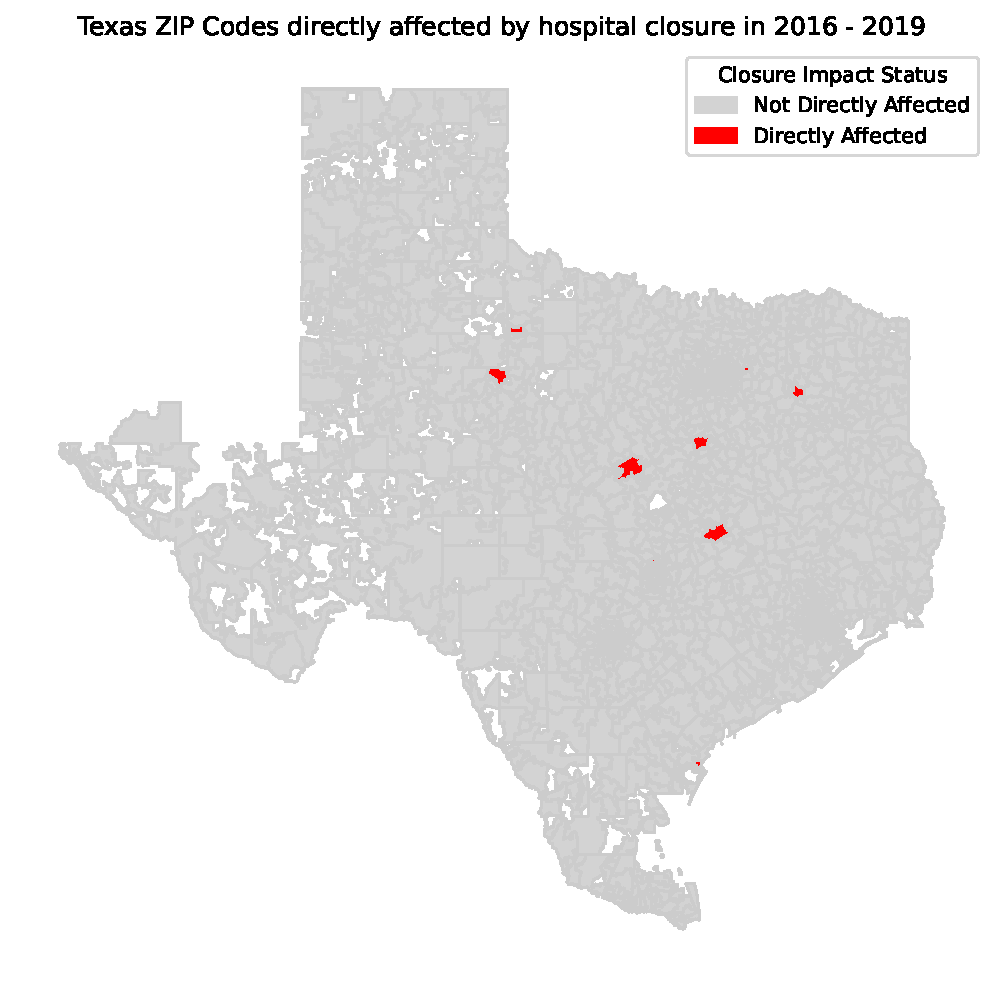
\includegraphics{pset4_template_files/figure-pdf/cell-30-output-1.pdf}

\begin{enumerate}
\def\labelenumi{\arabic{enumi}.}
\setcounter{enumi}{2}
\tightlist
\item
\end{enumerate}

\begin{Shaded}
\begin{Highlighting}[]
\CommentTok{\# create a GeoDataFrame of the directly affected zip codes}
\NormalTok{directly\_affected\_zips }\OperatorTok{=}\NormalTok{ closed\_hospitals\_tx\_zip\_merged[closed\_hospitals\_tx\_zip\_merged[}\StringTok{\textquotesingle{}directly affected\textquotesingle{}}\NormalTok{] }\OperatorTok{==} \DecValTok{1}\NormalTok{].copy()}

\NormalTok{directly\_affected\_zips }\OperatorTok{=}\NormalTok{ directly\_affected\_zips[[}\StringTok{\textquotesingle{}ZIP\_CD\textquotesingle{}}\NormalTok{, }\StringTok{\textquotesingle{}geometry\textquotesingle{}}\NormalTok{]]}

\BuiltInTok{print}\NormalTok{(}\StringTok{\textquotesingle{}Check if the object is a GepDataFrame:\textquotesingle{}}\NormalTok{, }\BuiltInTok{type}\NormalTok{(directly\_affected\_zips))}
\end{Highlighting}
\end{Shaded}

\begin{verbatim}
Check if the object is a GepDataFrame: <class 'geopandas.geodataframe.GeoDataFrame'>
\end{verbatim}

\begin{Shaded}
\begin{Highlighting}[]
\CommentTok{\# geopandas uses meters to creat buffer, check the unit for our GeoDataFrame}
\NormalTok{directly\_affected\_zips.crs}
\CommentTok{\# create a list of directly affected zip codes}
\NormalTok{directly\_affected\_zips\_list }\OperatorTok{=}\NormalTok{ directly\_affected\_zips[}\StringTok{\textquotesingle{}ZIP\_CD\textquotesingle{}}\NormalTok{].unique().tolist()}

\CommentTok{\# create a copy and convert into crs for Texas that is in meters}
\NormalTok{directly\_affected\_buffer }\OperatorTok{=}\NormalTok{ directly\_affected\_zips.copy()}
\NormalTok{directly\_affected\_buffer }\OperatorTok{=}\NormalTok{ directly\_affected\_buffer.to\_crs(epsg}\OperatorTok{=}\DecValTok{3083}\NormalTok{)}

\CommentTok{\# create a 10{-}mile buffer by converting into meters}
\NormalTok{directly\_affected\_buffer[}\StringTok{\textquotesingle{}10{-}mile radius\textquotesingle{}}\NormalTok{] }\OperatorTok{=}\NormalTok{ directly\_affected\_buffer.geometry.}\BuiltInTok{buffer}\NormalTok{(}
    \DecValTok{10}\OperatorTok{*}\FloatTok{1609.34}\NormalTok{)}
\NormalTok{directly\_affected\_buffer }\OperatorTok{=}\NormalTok{ directly\_affected\_buffer.set\_geometry(}
    \StringTok{\textquotesingle{}10{-}mile radius\textquotesingle{}}\NormalTok{)}
\end{Highlighting}
\end{Shaded}

\begin{Shaded}
\begin{Highlighting}[]
\CommentTok{\# before doing spatial join, ensure the overall Texas ZIP shapefile is in the same crs}
\NormalTok{zip\_tx }\OperatorTok{=}\NormalTok{ zip\_tx.to\_crs(epsg}\OperatorTok{=}\DecValTok{3083}\NormalTok{)}

\CommentTok{\# do the spatial join which will return all directly and indirectly affected zip codes}
\NormalTok{indirectly\_affected\_zips }\OperatorTok{=}\NormalTok{ gpd.sjoin(zip\_tx, directly\_affected\_buffer,}
\NormalTok{                                     how}\OperatorTok{=}\StringTok{"inner"}\NormalTok{, predicate}\OperatorTok{=}\StringTok{\textquotesingle{}intersects\textquotesingle{}}\NormalTok{)}

\CommentTok{\# rename ZIP\_CD\_left to \textquotesingle{}ZIP\_CD\textquotesingle{} for indirectly affected zips GeoDataFrame and set geometry back to geometry}
\NormalTok{indirectly\_affected\_zips }\OperatorTok{=}\NormalTok{ indirectly\_affected\_zips.rename(}
\NormalTok{    columns}\OperatorTok{=}\NormalTok{\{}\StringTok{\textquotesingle{}ZIP\_CD\_left\textquotesingle{}}\NormalTok{: }\StringTok{\textquotesingle{}ZIP\_CD\textquotesingle{}}\NormalTok{\})}

\CommentTok{\# create a list of only indirectly affected zip codes}
\NormalTok{indirectly\_affected\_zips\_list }\OperatorTok{=}\NormalTok{ indirectly\_affected\_zips[}\StringTok{\textquotesingle{}ZIP\_CD\textquotesingle{}}\NormalTok{].unique().tolist()}

\NormalTok{indirectly\_affected\_zips\_list }\OperatorTok{=}\NormalTok{ [}
\NormalTok{    zip\_code }\ControlFlowTok{for}\NormalTok{ zip\_code }\KeywordTok{in}\NormalTok{ indirectly\_affected\_zips\_list}
    \ControlFlowTok{if}\NormalTok{ zip\_code }\KeywordTok{not} \KeywordTok{in}\NormalTok{ directly\_affected\_zips\_list}
\NormalTok{]}

\BuiltInTok{print}\NormalTok{(}\StringTok{\textquotesingle{}There are\textquotesingle{}}\NormalTok{, }\BuiltInTok{len}\NormalTok{(indirectly\_affected\_zips\_list),}
      \StringTok{\textquotesingle{}indirectly affected zip codes in Texas\textquotesingle{}}\NormalTok{)}

\CommentTok{\# set geometry back to the original geometry column}
\NormalTok{indirectly\_affected\_zips }\OperatorTok{=}\NormalTok{ indirectly\_affected\_zips.set\_geometry(}\StringTok{\textquotesingle{}geometry\textquotesingle{}}\NormalTok{)}
\end{Highlighting}
\end{Shaded}

\begin{verbatim}
There are 342 indirectly affected zip codes in Texas
\end{verbatim}

\begin{enumerate}
\def\labelenumi{\arabic{enumi}.}
\setcounter{enumi}{3}
\tightlist
\item
\end{enumerate}

\begin{Shaded}
\begin{Highlighting}[]
\CommentTok{\# create a column representing Hospital Closures Impact Status}
\NormalTok{closed\_hospitals\_tx\_zip\_merged[}\StringTok{\textquotesingle{}Closure Impact Status\textquotesingle{}}\NormalTok{] }\OperatorTok{=} \StringTok{\textquotesingle{}Not Affected\textquotesingle{}}
\NormalTok{closed\_hospitals\_tx\_zip\_merged.loc[closed\_hospitals\_tx\_zip\_merged[}\StringTok{\textquotesingle{}ZIP\_CD\textquotesingle{}}\NormalTok{].isin(}
\NormalTok{    directly\_affected\_zips\_list), }\StringTok{\textquotesingle{}Closure Impact Status\textquotesingle{}}\NormalTok{] }\OperatorTok{=} \StringTok{\textquotesingle{}Directly Affected\textquotesingle{}}
\NormalTok{closed\_hospitals\_tx\_zip\_merged.loc[closed\_hospitals\_tx\_zip\_merged[}\StringTok{\textquotesingle{}ZIP\_CD\textquotesingle{}}\NormalTok{].isin(}
\NormalTok{    indirectly\_affected\_zips\_list), }\StringTok{\textquotesingle{}Closure Impact Status\textquotesingle{}}\NormalTok{] }\OperatorTok{=} \StringTok{\textquotesingle{}Indirectly Affected\textquotesingle{}}
\BuiltInTok{print}\NormalTok{(closed\_hospitals\_tx\_zip\_merged[}\StringTok{\textquotesingle{}Closure Impact Status\textquotesingle{}}\NormalTok{].value\_counts())}
\end{Highlighting}
\end{Shaded}

\begin{verbatim}
Closure Impact Status
Not Affected           1579
Indirectly Affected     342
Directly Affected        14
Name: count, dtype: int64
\end{verbatim}

\begin{Shaded}
\begin{Highlighting}[]
\CommentTok{\# create a color map for different impact status}
\NormalTok{color\_map }\OperatorTok{=}\NormalTok{ \{}
    \StringTok{\textquotesingle{}Directly Affected\textquotesingle{}}\NormalTok{: }\StringTok{\textquotesingle{}red\textquotesingle{}}\NormalTok{,}
    \StringTok{\textquotesingle{}Indirectly Affected\textquotesingle{}}\NormalTok{: }\StringTok{\textquotesingle{}orange\textquotesingle{}}\NormalTok{,}
    \StringTok{\textquotesingle{}Not Affected\textquotesingle{}}\NormalTok{: }\StringTok{\textquotesingle{}lightgray\textquotesingle{}}
\NormalTok{\}}

\CommentTok{\# plot a choropleth}
\NormalTok{fig, ax }\OperatorTok{=}\NormalTok{ plt.subplots(figsize}\OperatorTok{=}\NormalTok{(}\DecValTok{10}\NormalTok{, }\DecValTok{8}\NormalTok{))}
\NormalTok{closed\_hospitals\_tx\_zip\_merged.plot(}
\NormalTok{    column}\OperatorTok{=}\StringTok{\textquotesingle{}Closure Impact Status\textquotesingle{}}\NormalTok{,}
\NormalTok{    color}\OperatorTok{=}\NormalTok{closed\_hospitals\_tx\_zip\_merged[}\StringTok{\textquotesingle{}Closure Impact Status\textquotesingle{}}\NormalTok{].}\BuiltInTok{map}\NormalTok{(}
\NormalTok{        color\_map),}
\NormalTok{    edgecolor}\OperatorTok{=}\StringTok{\textquotesingle{}0.8\textquotesingle{}}\NormalTok{,}
\NormalTok{    legend}\OperatorTok{=}\VariableTok{True}\NormalTok{,}
\NormalTok{    ax}\OperatorTok{=}\NormalTok{ax}
\NormalTok{)}

\CommentTok{\# create a custom legend}
\NormalTok{patches }\OperatorTok{=}\NormalTok{ [mpatches.Patch(color}\OperatorTok{=}\NormalTok{color, label}\OperatorTok{=}\NormalTok{status)}
           \ControlFlowTok{for}\NormalTok{ status, color }\KeywordTok{in}\NormalTok{ color\_map.items()]}
\NormalTok{ax.legend(handles}\OperatorTok{=}\NormalTok{patches, title}\OperatorTok{=}\StringTok{"Closure Impact Status"}\NormalTok{,}
\NormalTok{          loc}\OperatorTok{=}\StringTok{\textquotesingle{}lower center\textquotesingle{}}\NormalTok{, bbox\_to\_anchor}\OperatorTok{=}\NormalTok{(}\FloatTok{0.5}\NormalTok{, }\OperatorTok{{-}}\FloatTok{0.05}\NormalTok{), ncol}\OperatorTok{=}\DecValTok{3}\NormalTok{)}

\NormalTok{ax.set\_axis\_off()}
\NormalTok{plt.title(}\StringTok{\textquotesingle{}Impact Status of Hospital Closures in Texas (2016{-}2019)\textquotesingle{}}\NormalTok{)}
\NormalTok{plt.show()}
\end{Highlighting}
\end{Shaded}

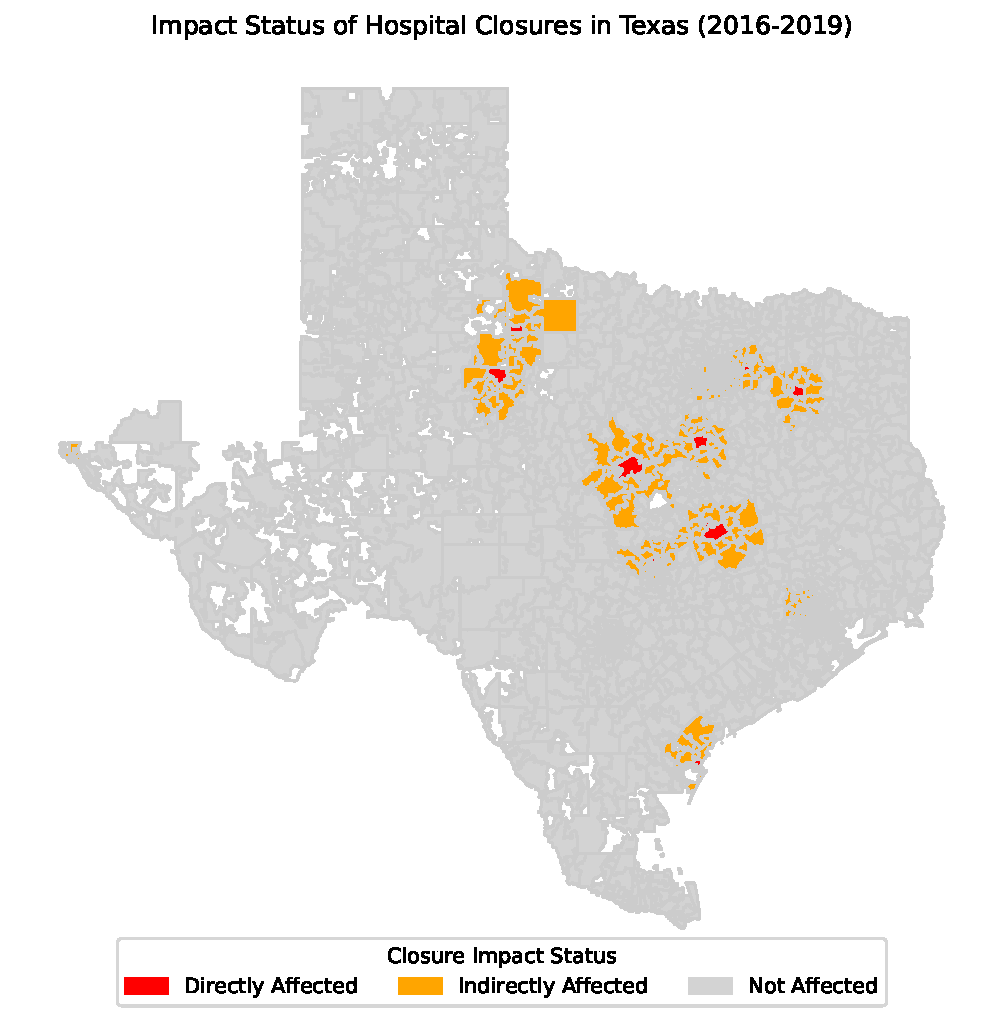
\includegraphics{pset4_template_files/figure-pdf/cell-35-output-1.pdf}

\subsection{Reflecting on the exercise (10
pts)}\label{reflecting-on-the-exercise-10-pts}

\begin{enumerate}
\def\labelenumi{\arabic{enumi}.}
\item
  There are some deficiencies in the method. In Section 2, when
  attempting to identify `false closures,' we removed zip codes where
  the number of active hospitals in the closure year did not decrease in
  subsequent years. However, this approach only partially addresses the
  possibility of mergers. Since the count of active hospitals in the
  closure year does not include the hospitals that closed, the number
  may remain stable in the following year even if no merger or
  acquisition occurred. This means we may have mistakenly excluded some
  zip codes with actual closures. To improve, we could consider to
  compare the number of active hospitals in the year before the closure
  to the year after the closure. This would help us identify potential
  mergers more accurately, as it accounts for changes in hospital
  availability over a broader period.
\item
  This method can partially reflect changes in the hospital access due
  to hospital closures especially if that particular zip-code already
  has a lower access, that is low amount of hospitals in the zip code.
  Otherwise, they might not be affected much by a hospital closure. Same
  as indirectly affected zip codes, they might not be affected at all if
  there are other hospitals in their areas. So we should also consider
  existing hospitals density in that zip code and neighboring zip codes
  as well. Another thing to consider is the share of patients that the
  closed hospitals have in the zip-code level. Also, the change in
  travel distance to nearest hospital in the zip code could tell us more
  about the actual impact on that zip code.
\end{enumerate}




\end{document}
